\documentclass[twocolumn]{article}
\usepackage[utf8]{inputenc}
\usepackage[english]{babel}
% \usepackage[left=2.5cm,right=2.5cm,top=3cm,bottom=3cm]{geometry}
\usepackage[T1]{fontenc}
\usepackage[os=mac, mackeys=symbols]{menukeys}
\usepackage{graphicx}
\graphicspath{{plots/}{../img/}{tegninger/}}
\usepackage{xspace}
\usepackage[noadjust]{cite}
\usepackage{caption}
\usepackage{subcaption}
\usepackage{booktabs}
\usepackage{cancel}
\usepackage{subcaption}
\usepackage{float}
\usepackage{amsmath}
\usepackage{enumerate} % bedre enumeration
\usepackage{enumitem}
\usepackage{amssymb}
\usepackage{amsthm}
\usepackage{makecell}
\usepackage{algorithm}
\usepackage{algpseudocode}
\usepackage{listings}
\usepackage{minted}
\usepackage[all]{xy}
\usepackage[hidelinks]{hyperref}
\usepackage[nameinlink,noabbrev]{cleveref}

\lstset{
    language=C++,
    basicstyle=\ttfamily,
    keywordstyle=\color{blue}\ttfamily,
    stringstyle=\color{red}\ttfamily,
    commentstyle=\color{gray}\ttfamily,
    morecomment=[l][\color{magenta}]{\#},
    showstringspaces=false,
    numbers=left,
    tabsize=2,
    breaklines=true,
    breakatwhitespace=false,
}

\lstset
{ %Formatting for code in appendix
    % basicstyle=\footnotesize,
    numbers=left,
    stepnumber=1,
    showstringspaces=false,
    tabsize=2,
    breaklines=true,
    breakatwhitespace=false,
}
\usepackage{cite}
\usepackage{mathtools}
\usepackage{pdfpages}
% \usepackage[framemethod=TikZ]{mdframed}
% \mdfdefinestyle{TLO}{
%     innertopmargin=\baselineskip,
%     innerbottommargin=\baselineskip,
%     innerrightmargin=20pt,
%     innerleftmargin=20pt,}
% \usepackage[parfill]{parskip}  % ingen indent ved ny paragraf

\DeclarePairedDelimiter\ceil{\lceil}{\rceil}
\DeclarePairedDelimiter\floor{\lfloor}{\rfloor}
\DeclareMathOperator{\EX}{\mathbb{E}}
\DeclareMathOperator{\prob}{P}
\DeclareMathOperator{\RR}{\mathbb{R}}
\DeclareMathOperator{\NN}{\mathbb{N}}
\DeclareMathOperator{\CC}	{\mathbb{C}}
\DeclareMathOperator{\ZZ}{\mathbb{Z}}
\newcommand{\abs}[1]{\left|#1\right|}
\newcommand{\brac}[1]{\left\{#1\right\}}
\newcommand{\sqrbrac}[1]{\left[#1\right]}
\newcommand{\paren}[1]{\left(#1\right)}
\newcommand{\normlines}[1]{\left\Vert#1\right\Vert}
\newcommand{\mtx}[1]{\textbf{#1}}

\newcommand{\note}[1]{\textcolor{red}{#1}\\}

%%% FORMATTING %%%
\usepackage{enumitem}
\usepackage{titlesec}
\titlespacing*{\section}{0pt}{0.8\baselineskip}{0.3\baselineskip}
\titlespacing*{\subsection}{0pt}{0.4\baselineskip}{0.15\baselineskip}
\titleformat{\section}
  {\normalfont\Large\bfseries}{\thesection}{1em}{}
\titleformat{\subsection}
  {\normalfont\large\bfseries}{\thesubsection}{1em}{}

\usepackage{titling}
\setlength{\droptitle}{-6em} 
\setlength{\columnsep}{0.55in}

\usepackage{multirow}

\usepackage{fancyhdr}
\usepackage{lastpage}

\pagestyle{fancy}
\fancyhf{}
\rfoot{\centering Page \thepage \hspace{1pt} of \pageref{LastPage}}

\usepackage[a4paper,
            bindingoffset=0.2in,
            left=0.85in,
            right=0.85in,
            top=1.5in,
            bottom=1.5in,
            footskip=.25in]{geometry}

%%% TITLE%%%
\title{A Single Pass Scan Using Lookback}
\author{dwp992 \& lsh789}
\date{November 2023\vspace{2ex}}

\begin{document}

\maketitle
\thispagestyle{fancy}

\section{Introduction}
Throughout this course we've covered many topics in parallel programming, among these one of the primary building blocks of parallel programming: The array scan. The scanning algorithms we've seen up until now have either been fully sequential or have in some way been multi-pass, i.e., more than 2 reads/writes are made to global memory per element. In this project we seek to implement a parallel single pass scanning algorithm, utilizing shared memory and registers for the vast amount of our computations and only performing computations in global memory when doing inter-block computations. We experiment with different methods, such as having this inter-block communication being performed using an auxiliary block and using global aggregate and prefix arrays with blocks computing prefixes either sequential or in parallel. Furthermore, using these methods along with a list of baselines we experiment with different block sizes, register sizes per thread, and array size.

\section{Background}
\label{sec:background}

This project is based on the paper "Single-pass Parallel Prefix Scan with Decoupled Look-back" \cite{SPS_paper}. In this paper the authors go through explaining their implementation of a single pass scan, meaning we can scan with only 2 global IO accesses per element. (Not counting a few extra needed per block). The important part of the algorithm they introduce, is the decoupled lookback scan, that will scan over what previous blocks have gotten. The paper also proposes a number of optimisations, some of then we implemented and some of them will be discussed later on.

\subsection{Decoupled lookback}

Normally when we would do a scan we would need 3 global IO accesses per element, since we would first need a read, when calculating the reduction of each block and scanning over the result of these, this result will then be used in a second pass through were we then scan each block while adding the prefix we found from the reduction/block-level-scan this gives us another global read. And finally we need to write the result. What we can see from this normal implementation is that we 2 of the 3 global accesses are reading the same memory, the only problem is that we are reading it with bad temporal locality, so we can not keep the data. This is what we try to fix by doing a single-pass scan, since we only pass through the data once, we only do one global read. And then we calculate the reduction and result right away.

One of the issues with this way of implementing it. Is that we now have a dependency between the blocks, so in order for block 2 to calculate the result of it's scan, it needs the prefix value from block 1. In the paper they then introduce the lookback algorithm that lets the blocks update a global array with their prefix and aggregate values that future blocks then can use. This is done by the aggregate value being just a reduction of all the values in the block, and the prefix can be found by adding this aggregate to the previous blocks prefix. But for this we also need to ensure that the blocks are being calculated in certain order, so we do not just have all calculating threads waiting for block 1, that is in queue to being spawned, the paper suggest a dynamic scheduling of the blocks, which we utilised in our implementation.

\note{Bør man gå mere i dybden med aggrgate flag og prefix array, og lave en helt down to earth definition af dem : Jeg synes bare vi skal gøre det kort.}

\note{Maybe add the some text about the properties discussed in the paper, and what effect they have.}

\section{Our implementation}
\label{Sec:Implementation}
This section describes the lookback algorithm we've implemented, the kernel that executes the scan, and the associated functions we've defined. Listing \ref{lst:lookbackKernel} describes the lookback kernel and listing \ref{let:seqLookbackScan} contains the code for our lookback algorithm. All our kernel related code can be found in the \verb|spsKernels.cu.h| file, and our tests which verify the algorithms can be found in the \verb|testSPS.cu| file. The algorithms we've implemented verify against a sequential CPU scan, and using the accompanying code, while in the \verb|/src| directory, one can execute the code that verifies the algorithms by calling \verb|make|.

\subsection{The Lookback Scan Kernel}
\label{sec:impl-lookback-kernel}
Listing \ref{lst:lookbackKernel} takes pointers to the input and output arrays, along with a size. We also pass as arguments 4 pointers to different global memory locations. The first is a dynamic ID that is shared across blocks. The second, third, and fourth are pointers to the flag array, aggregate array, and inclusive prefix array described in section \ref{sec:background}. The arrays are implemented using the \verb|volatile| keyword to ensure that memory is visible for all threads as soon as it's written, and the dynamic ids are handled using atomic additions. Specifically, the \verb|atomicAdd| function is used to add to the global variable and return the value before adding. Line 9-10 initializes the shared memory that we'll need. We create a shared array of size $Q * B$ and a shared buffer of size $B$. The shared array accompanying each block is reserved for part of the array the block scans. The shared buffer stores scans performed by each thread on \verb|Q| elements. The kernel code contains 6 different device functions:
\begin{enumerate}[leftmargin=*]
    \itemsep0em
    \item \verb|copyGlb2Shr| - Copies memory from global to shared memory in a coalesced fashion. Equivalent to the function used in assignment 2.
    \item \verb|threadScan| - Each thread scans $Q$ elements from the shared memory and writes the resulting value to the shared buffer at the index equal to the thread id.
    \item \verb|blockScan| - Performs an inclusive scan equivalent to the optimized warp scan from assignment 2.
    \item \verb|threadAdd| - Adds the correct inclusive prefix to all values in the shared memory. After this function call, all values in shared memory have values representing an inclusive scan for the block only.
    \item \verb|lookbackScan| - The lookback scan function looks through the flag, aggregate and prefix arrays to compute the appropriate exclusive prefix to add to the respective blocks shared memory. This function is described in detail in subsection \ref{sec:impl-lookback-alg}.
    \item \verb|threadAddVal| - Each thread adds the appropriate exclusive prefix to the $Q$ elements it's responsible for.
    \item \verb|copyShr2Glb| - Copies the shared memory to a location in the global array in a coalesced fashion. This is functionally equivalent to the one we used in assignment 2.
\end{enumerate}

Originally the design choice to use a separate shared memory buffer was made as it made the algorithm easier to construct in pseudo code. Furthermore, this choice makes the whole algorithm more easy to understand and explain. A potential drawback could be inefficiency in using $B*4$ extra bytes of shared memory per block, since if $B=1024$, this shared buffer would use $4*1024/49152 = 0.083\approx 8\%$ of the shared memory per block.

\subsection{The Lookback Algorithm}
\label{sec:impl-lookback-alg}

In accordance with section \ref{sec:background} we have implemented the lookback algorithm using 3 different arrays in global memory: A flag array, an aggregate array, and an inclusive prefix array. this section covers the lookback version where only 1 thread computes the exclusive prefix and updates its own aggregate value and inclusive prefix values. The implementation of this can be seen in listing \ref{let:seqLookbackScan}. The lines 11 to 34 are computed only for the final thread in the block.

Line 11-16 covers the case in which the dynamic id is 0 - We set both the aggregate value and the prefix value equal to the final value in the shared memory for the block. It then memory fences and then sets its flag to be P.

Line 18-34 covers the cases where the dynamic ids are greater than 0. First the aggregate value is set to the final value in the shared memory for the block. After a memory fence we set the flag value to A. We then define a \verb|grab_id| - an index of where we want values to add to our current aggregate value to produce an inclusive prefix. In line 25-29, while the flag at \verb|grab_id| is not P and the \verb|grab_id| is greater than zero, the aggregate value at \verb|grab_id| is added to an accumulating variable and the id is decremented. Finally, once a P flag is reached, the prefix value at the dynamic id is set to the current accumulation plus the prefix value at the \verb|grab_id|. After a fence, set the dynamic id flag to P.

Finally after a inter-block thread synchronization, in line 37, computed by all threads in the block, a prefix variable is created - this is the exclusive prefix value returned. It is computed by the prefix value minus the aggregate value accompanying the dynamic id.

\subsection{Parallelization of the lookback algorithm}

\subsection{SPS using an auxiliary block}

We also implemented the method mentioned in the old slides written by professor Henriksen, wherein the construction of the inclusive prefix array is done by one auxiliary block that is given the dynamic id of -1. As values in the aggregate array become available, this auxiliary block sequentially computes the prefix array. Blocks that have computed an aggregate value wait for the prefix value to be computed, and once it has the block adds the exclusive prefix to its section of the scanned array.

\section{Throughput for different array sizes}
\label{sec:tp_diff_arr_sizes}
\subsection{Experiment}
Our first experiment focused on exploring how the throughput changed as we increased the array size. We measured throughput in terms of GB/s read/written to global memory on average over 100 runs for both GPU and CPU. For randomly initialized arrays of sizes between $2^{10}$ and $2^{30}$ we measure the performance of our implementations and some baseline computations. Our baseline computations are the \verb|cudaMemcpy|, a naive memcpy kernel, a sequential scan running on CPU, and the GPU inclusive scan algorithm from assignment 2. We measure the performance of our sequential lookback method, our modified parallel lookback method, and our implementation of single pass scan using an auxiliary block.

For these experiments we heuristically found the combinations $Q=30,B=256$, $Q=10, B=256$, and $Q=10,B=1024$ to achieve great results for all methods when compared to other parameters. Our intuition for why these parameters work will is that they utilize have greater of the shared memory available to each block, leading to an overall faster algorithm, as we can make many more computations in shared memory.

We expect to see the \verb|cudaMemcpy| and naive memcpy kernel to achieve the highest throughput, as it is the de facto high ceiling of how well our algorithm can perform. We expect the parallel lookback scan to outperform the sequential lookback scan, but that both of them would outperform the rest of the methods. We do expect the auxiliary method to fare worse than the lookback method but better than the GPU inclusive scan.

\subsection{Results}
The results of this experiment can be seen in figures \ref{fig:plot_256_30}, \ref{fig:plot_256_10}, and \ref{fig:plot_1024_10}. From all figures we can clearly see that \verb|cudaMemcpy| and our naive memcpy implementation achieved the highest throughput in the experiments, with one instance of \verb|cudaMemcpy| for $N=21$ in figure \ref{fig:plot_256_10} having a throughput of almost 1500 GB/s, nearing the theoretical limit of 1555 GB/s on the used hardware.

We see that in figures \ref{fig:plot_1024_10} and \ref{fig:plot_256_30} the parallel lookback outperforms all other scan methods tested, while in \ref{fig:plot_256_10} the baseline GPU scan outperforms both the parallel and sequential lookback scan. Our hypothesis for this is that as we lower batch size, the chunk size of the will increase accordingly for the baseline GPU scan, while for our lookback scan implementation suffers from smaller computations in shared memory, and more computations in global memory.

We also generally see that the auxiliary block version has performance similar to a sequential CPU scan. This was surprising to us as we assumed the mentioning of it in the supplementary slides indicated the solution. This very low throughput might be due to our implementation, but so far we haven't found the culprit.

Finally, from this data we can also measure the performance difference between our implementations and our baseline naive memcpy, which can be found in table \ref{tab:throughput_vs_naiveMemcpy}. We see first of all that the auxiliary block method clearly underperforms. At $b=256,Q=30$ we do however achieve 71\% of the throughput of memcpy for our sequential lookback, and 84\% of the throughput for our parallel lookback.

\begin{table}[h]
    \centering
    \begin{tabular}{lrrr}
        \toprule
         & \begin{tabular}{@{}c@{}}B=256\\Q=30\end{tabular} & \begin{tabular}{@{}c@{}}B=256\\Q=10\end{tabular} & \begin{tabular}{@{}c@{}}B=1024\\Q=10\end{tabular} \\
        \midrule
        naiveMemcpy & 1.00x & 1.00x & 1.00x \\
        SeqLookback & 0.71x & 0.34x & 0.61x \\
        ParLookback & 0.84x & 0.49x & 0.62x \\
        AuxBlock & 0.03x & 0.01x & 0.01x \\
        \bottomrule
    \end{tabular}
    \caption{Throughput performance vs naiveMemcpy}
    \label{tab:throughput_vs_naiveMemcpy}
\end{table}

\begin{figure}[h]
    \centering
    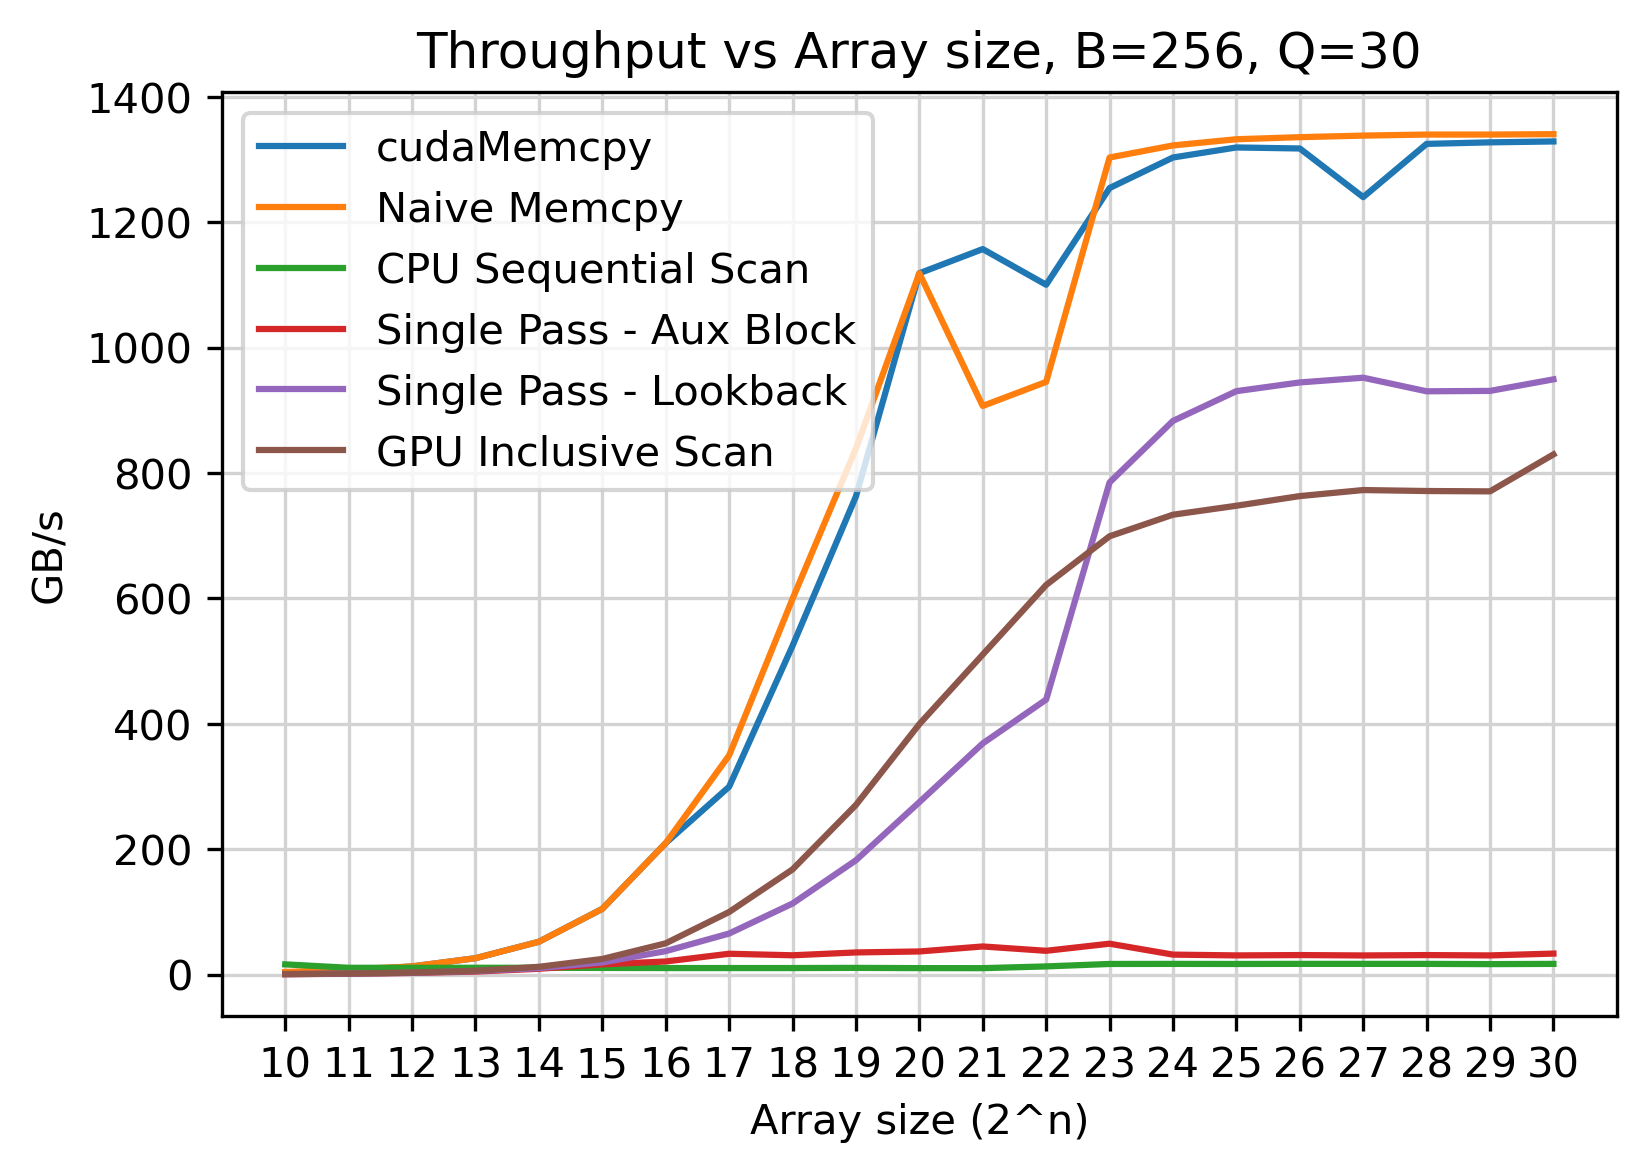
\includegraphics[width=\linewidth]{report/plots/throughput_vs_array_size_B256_Q30.png}
    \caption{throughput measurements for $B=256,Q=30$.}
    \label{fig:plot_256_30}
\end{figure}

\begin{figure}[h]
    \centering
    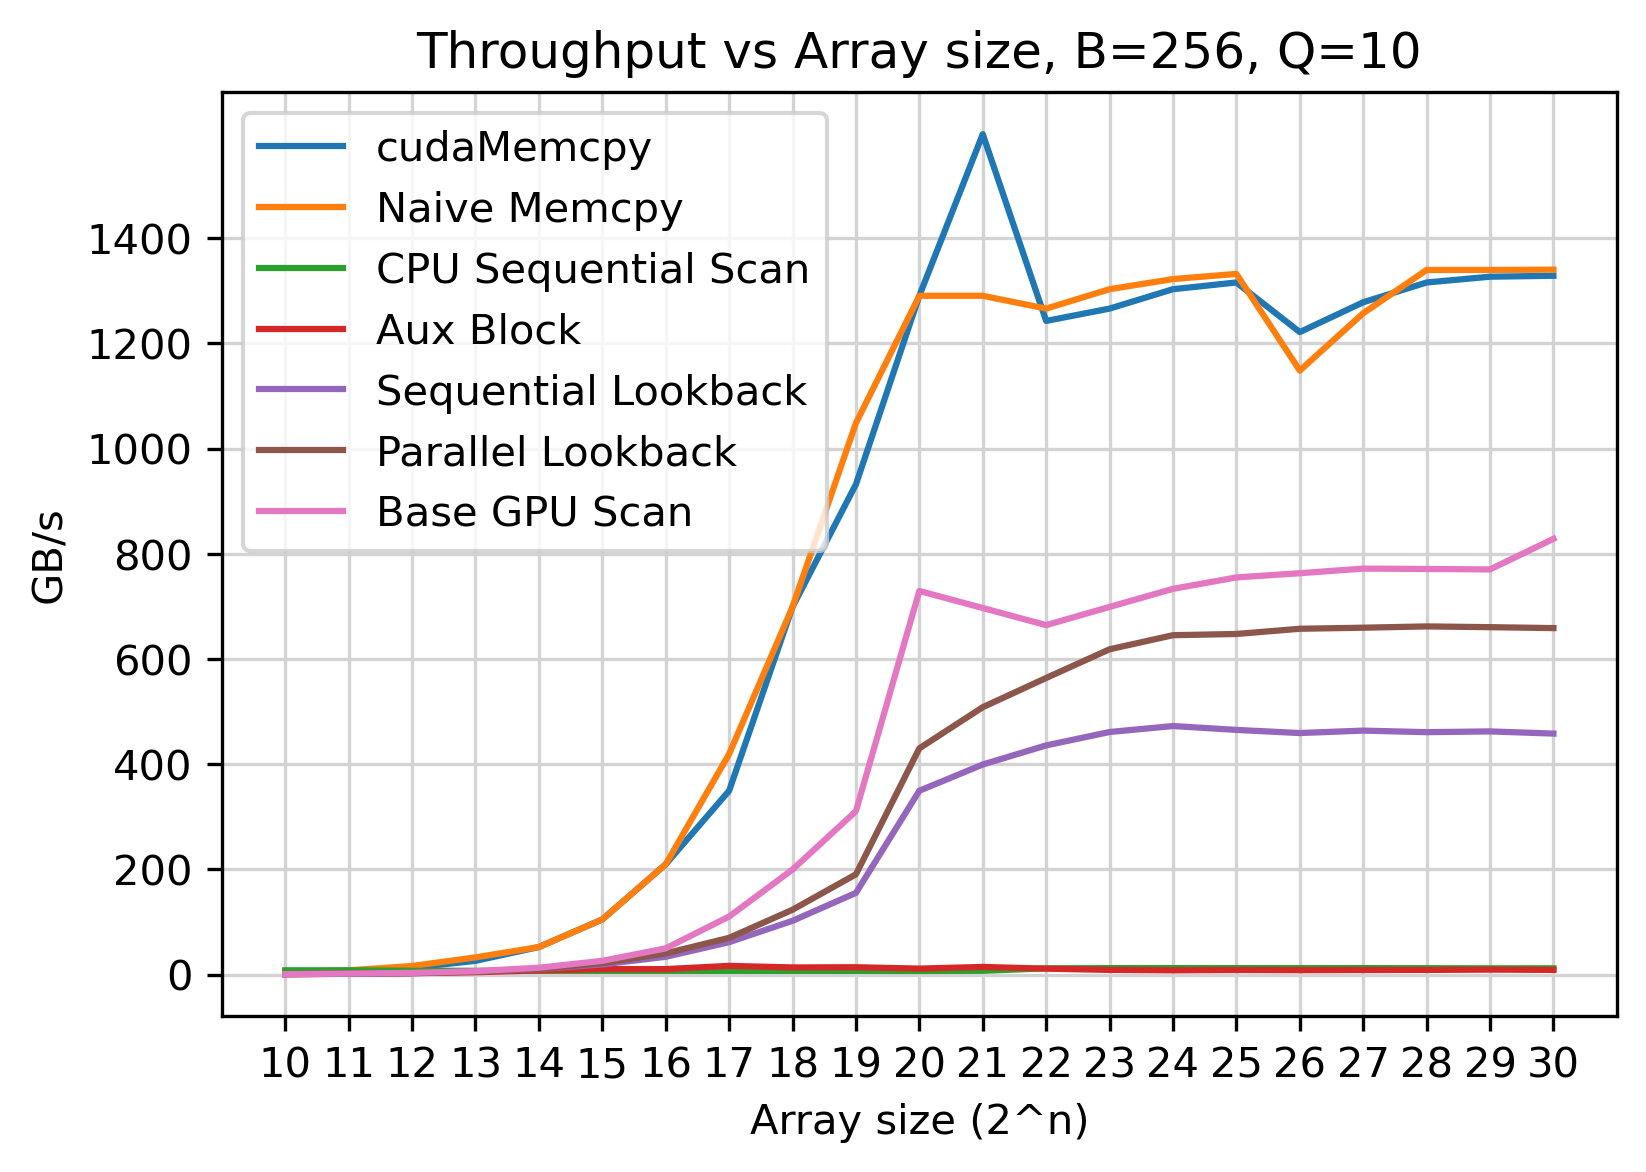
\includegraphics[width=\linewidth]{report/plots/throughput_vs_array_size_B256_Q10.png}
    \caption{throughput measurements for $B=256,Q=10$.}
    \label{fig:plot_256_10}
\end{figure}

\begin{figure}[h]
    \centering
    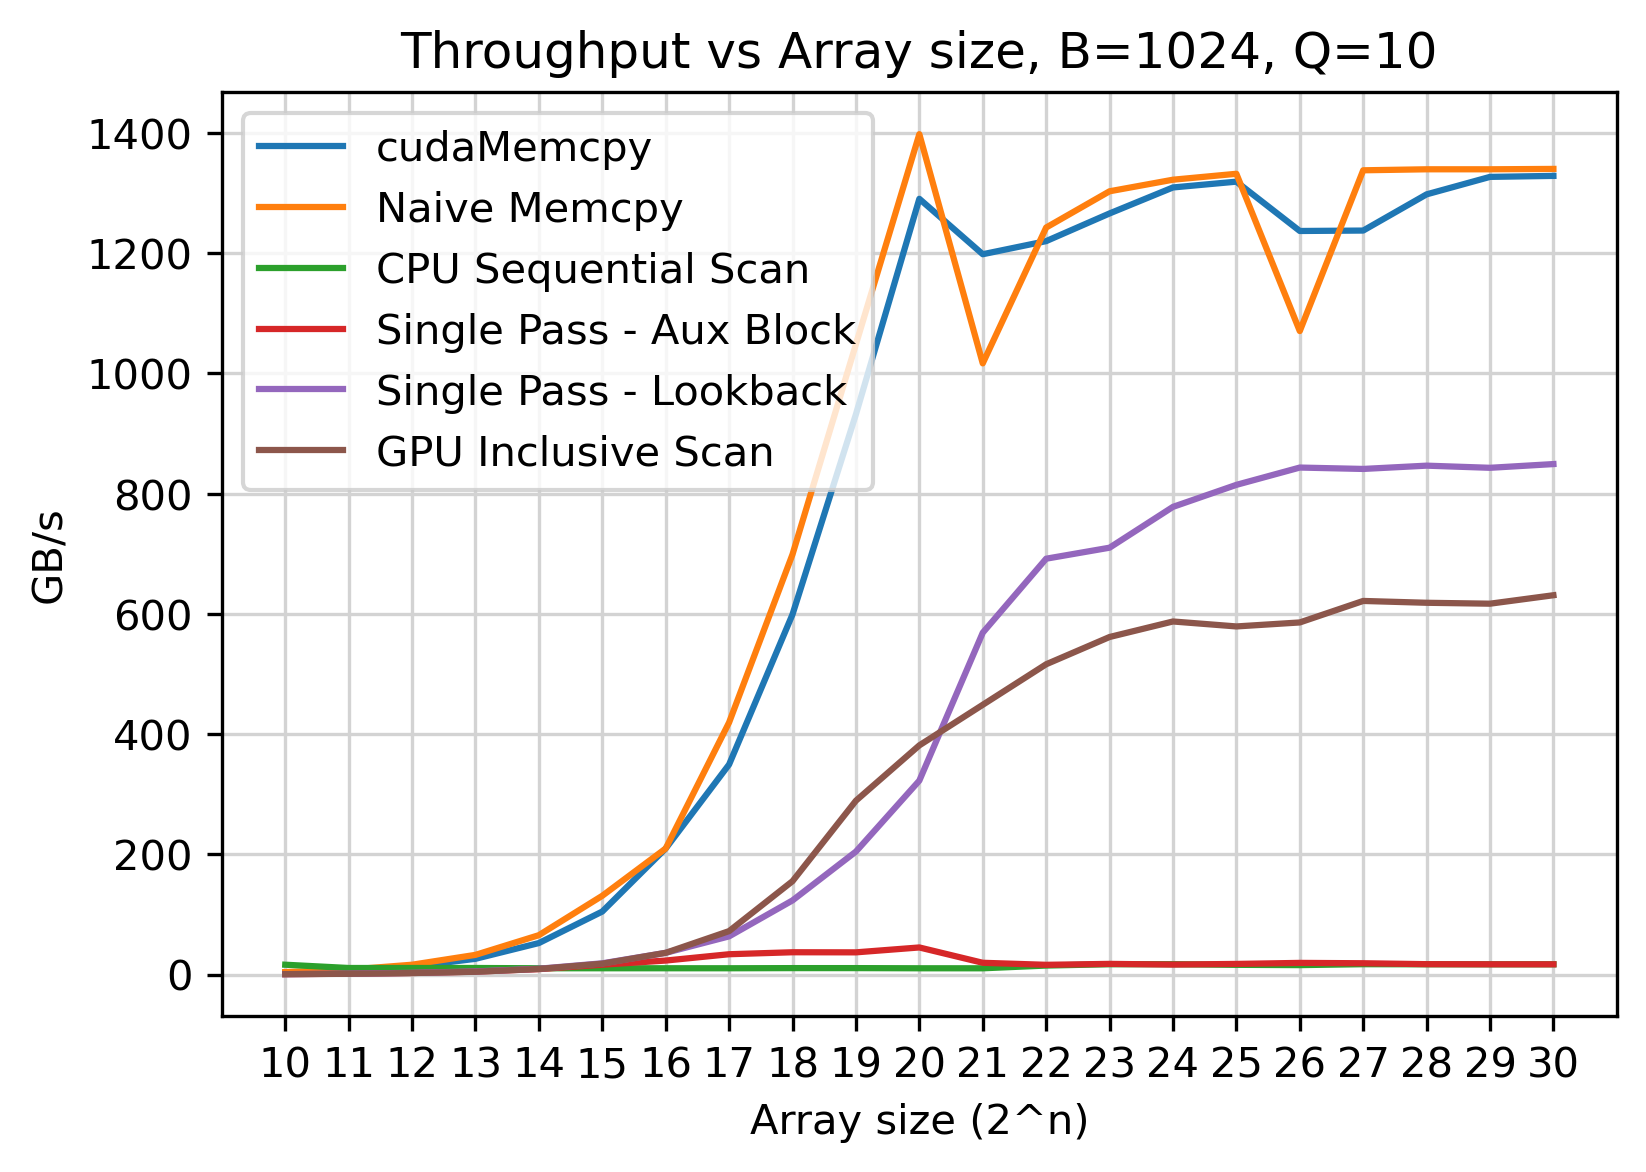
\includegraphics[width=\linewidth]{report/plots/throughput_vs_array_size_B1024_Q10.png}
    \caption{throughput measurements for $B=1024,Q=10$.}
    \label{fig:plot_1024_10}
\end{figure}

\section{Changes in throughput as we vary B, Q, and N}
\subsection{Experiments}
Our next experiment was to decide on lists of parameter values for each of $B$, $Q$, and $N$:
\begin{itemize}
    \item $B$: 2, 4, 7, 8, 10, 13, 16, 20, 24, 30, 32, 40.
    \item $Q$: 32, 64, 128, 256, 512, 1024.
    \item $N$: $2^i \; \forall \; i \in [10,30]$.
\end{itemize}
For each pairing of these parameters we computed the throughput of what we saw to be the best performing scan method we implemented - the parallel lookback scan. After this we found the highest throughput measured, which was $1133.64$ GB/s with the parameters $B=256,N=2^30,Q=30$. Using these values we created heatmaps of the three different slices created by fixing either of the parameters and varying the two others. These figures are found in figure \ref{fig:heatmaps}.

\subsection{Results}
\label{sec:results}
The heatmaps seen in figure \ref{fig:heatmaps} show that as we change each of parameters the change in throughput varies. In figure \ref{fig:heatmap-q} we see that as we increase $N$ but leave $Q$ fixed, apart form using a block size of 32 or 64 there isn't a large difference between the block sizes used. Furthermore, for lower $N$s there is little to no difference between throughput for different batch sizes.

We can see a similar pattern in figure \ref{fig:heatmap-b}: For lower $N$s there is a neglegible difference in throughput regardless of $Q$. As we increase $N$, the value of $Q$ becomes more important. After an array size of $2^20$ we start seeing throughput increases with Q and reaches the max measured throughput at $Q=30$. Most significantly, for some values ($Q=16,32$) we see a collapse in performance. This is due to the fact that shared memory in a block works in an interesting way. The reason for this low performance is that we are experiencing shared memory bank conflicts caused by the fact that each thread accesses shared memory through different memory banks, and the ids for these banks are computed by dividing the memory address by 32. Thus, by setting $Q=32$, all 32 reads/writes to shared memory performed by a thread is done sequentially as they all end up using the same memory bank.

In figure \ref{fig:heatmap-n} we see that varying $B$ changes the throughput measured more drastically than changing $Q$. While the range in $B$-values is shorter, even when making larger steps along the $Q$-values we don't see as drastic a change. Specifically, For any $Q\geq 10$ if we change the $Q$ the throughput stays relatively fixed, while a change in block size can alter the throughput noticeably. This is likely due to the fact that by increasing the block size we are simply able to revert many more computations away from global memory and into shared memory, and due to the fact that scanning inside a block is quite efficient with our implementation.

\begin{figure*}[h]
    \centering
    \begin{subfigure}{0.31\linewidth}
        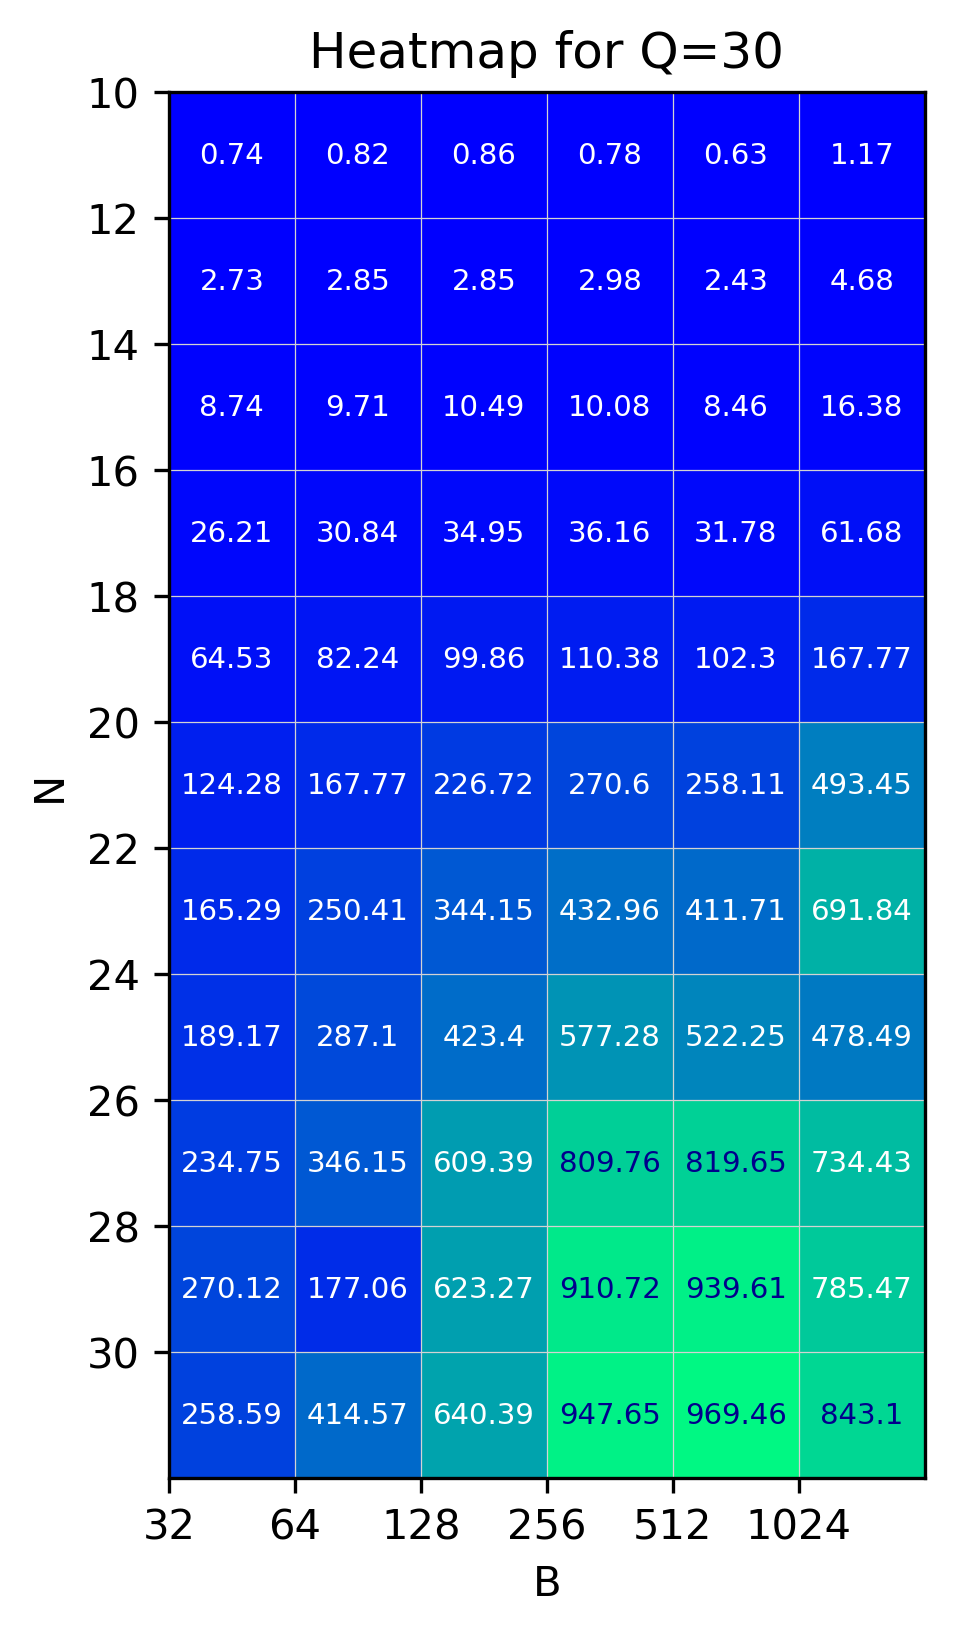
\includegraphics[width=\linewidth]{report/plots/heatmap_BvN_Q=30.png}
        \caption{Heatmap of different block sizes versus array length for $Q=30$.}
        \label{fig:heatmap-q}
    \end{subfigure}
    \begin{subfigure}{0.31\linewidth}
        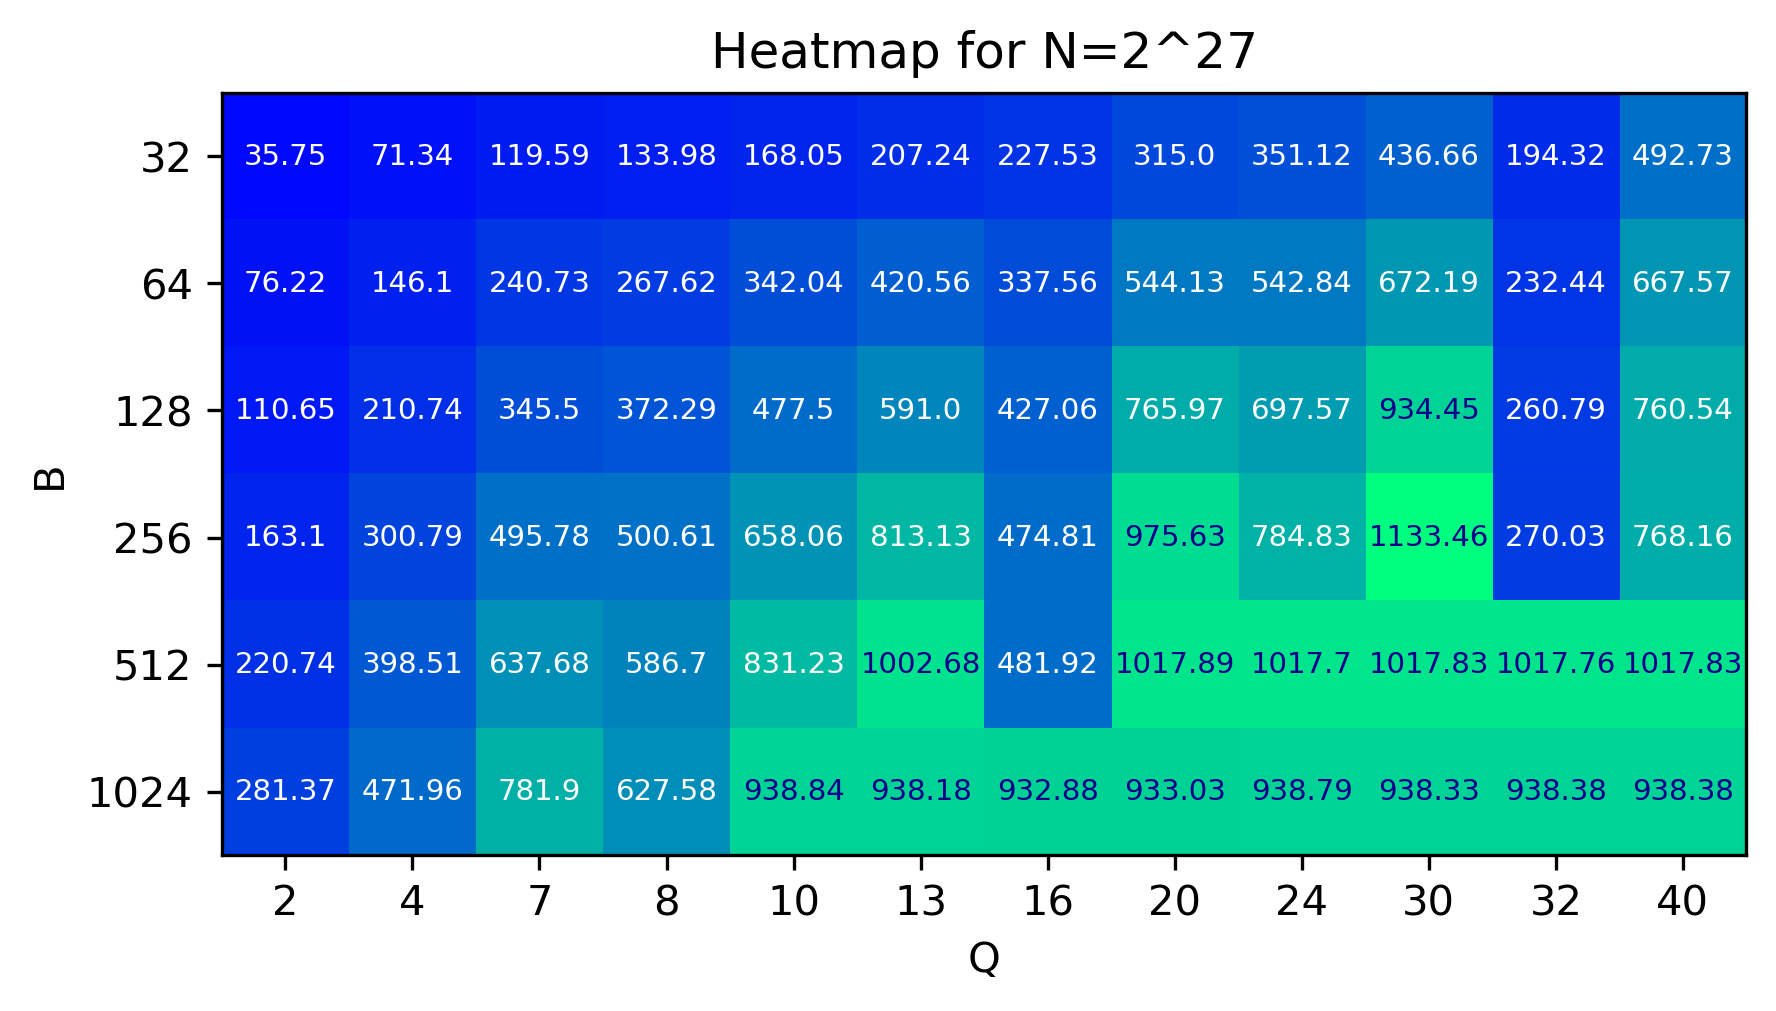
\includegraphics[width=\linewidth]{report/plots/heatmap_BvQ_N=28.png}
        \caption{Heatmap of different block sizes vs Q for array length $=2^{30}$}
        \label{fig:heatmap-n}
    \end{subfigure}
    \begin{subfigure}{0.68\linewidth}
        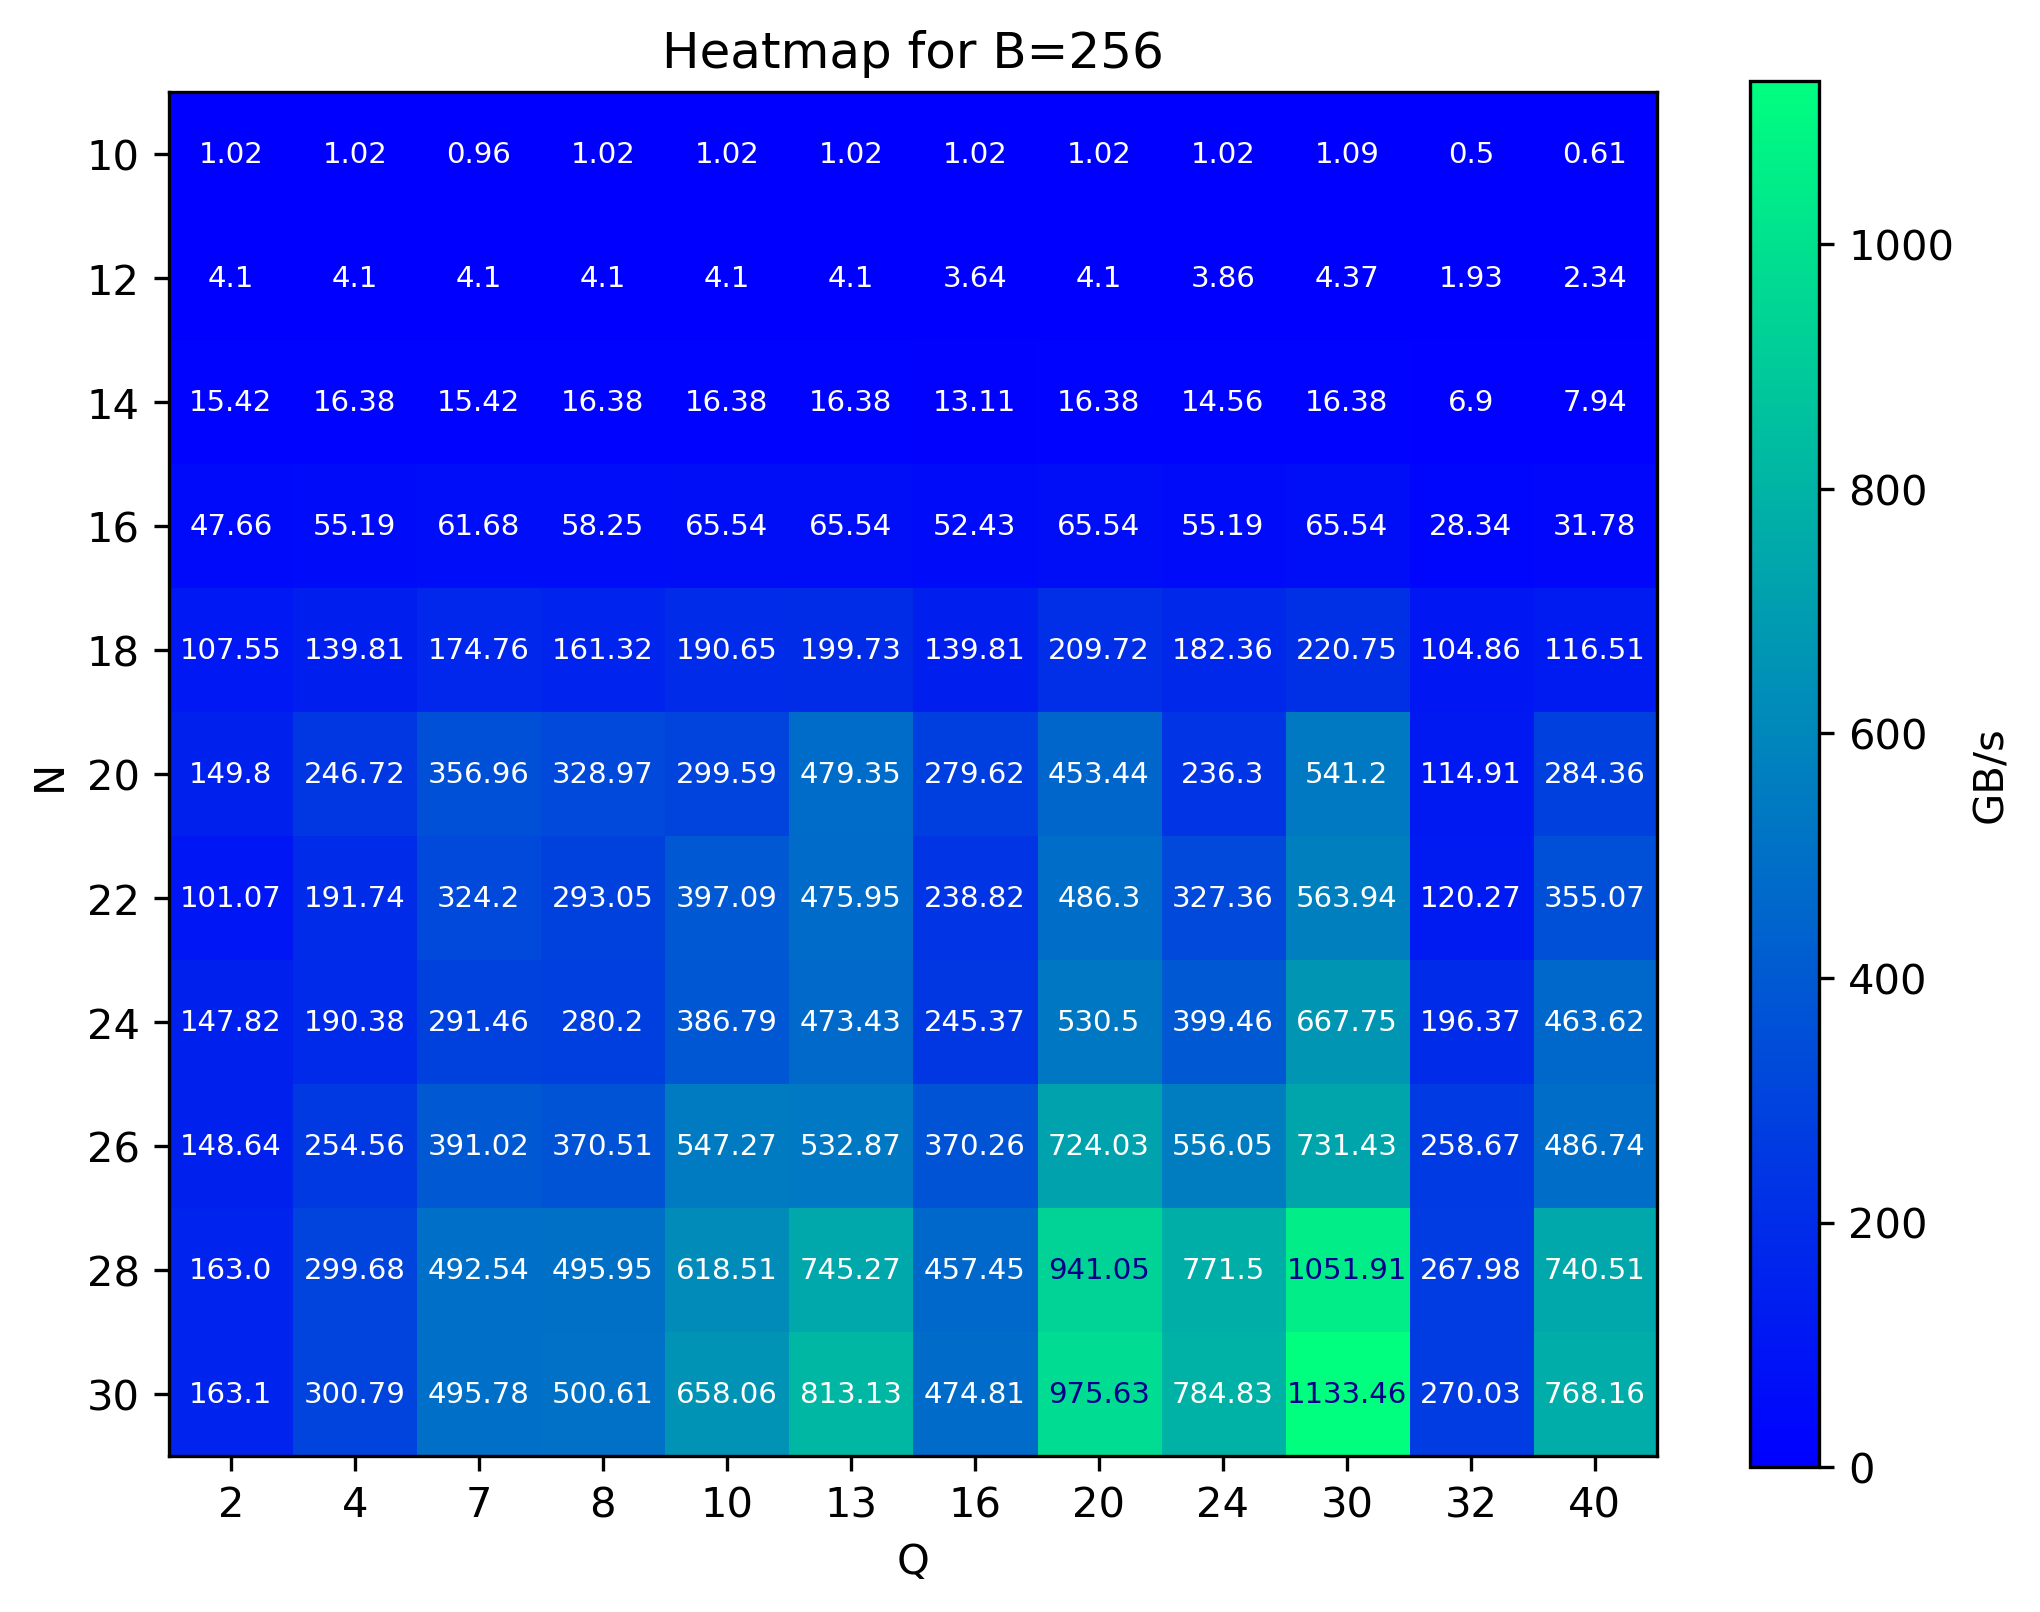
\includegraphics[width=\linewidth]{report/plots/heatmap_QvN_B=256.png}
        \caption{Heatmap of different Q's vs array length for block size $=256$}
        \label{fig:heatmap-b}
    \end{subfigure}
    \caption{Heatmaps made by fixing one of $Q, B, N$ and varying the others.}
    \label{fig:heatmaps}
\end{figure*}

\section{Conclusion}
This report covers our venture into implementing an efficient single pass scan. Utilizing shared memory and registers to handle intra-block scans, along with different methods of handling inter-block computations, we've implemented different single pass scan methods which we've experimented with. We've experimented with different block sizes, number of registers per thread, and the array size. We find that our implementations verify when compared to a basic sequential scan. We find that our implementation of parallel lookback scan achieves up to 84\% of the throughput of a naive memcpy implementation with a sequential implementation not far behind, and that our auxiliary block implementation achieves terrible results. The highest throughput we achieve is 1133.64 GB/s with a block size of 256 and a per thread register count of 30. We also find that Varying block size can be essential to the throughput of the method.

\section{Future work or future improvements}
\note{Not sure what this section should be named.}
\note{Remember to reference the idea we mentioned earlier about not using a shared buffer for blockScan.}

\onecolumn

\newpage

\bibliographystyle{plain} % We choose the "plain" reference style
\bibliography{refs} % Entries are in the refs.bib file

\section{Appendix}

\appendix

\section{Code for the sequential lookback scan function}
\begin{lstlisting}[caption=Lookback kernel,label=let:seqLookbackScan]
template<typename T>
__device__ inline T lookbackScan(volatile T* agg_mem,
                                 volatile T* pref_mem,
                                 volatile uint32_t* flag_mem,
                                 T* shr_mem, uint32_t dyn_idx,
                                 uint32_t tid) {
    #define X 0
    #define A 1
    #define P 2
	// Handle lookback differently depending on dynamic id.
    if (tid == B - 1 && dyn_idx == 0) {
		T agg_val = shr_mem[(Q - 1) * B + tid];
		agg_mem[dyn_idx] = agg_val;
        pref_mem[dyn_idx] = agg_val;
        __threadfence();
        flag_mem[dyn_idx] = P;

    } else if (tid == B - 1 && dyn_idx > 0) {
		T agg_val = shr_mem[(Q - 1) * B + tid];
        agg_mem[dyn_idx] = agg_val;
        __threadfence();
        flag_mem[dyn_idx] = A;
        uint32_t grab_id = dyn_idx - 1;
        // isnt there a bug here when we encounter an X?
        while (flag_mem[grab_id] != P) {
            if (flag_mem[grab_id] == A && grab_id > 0) {
                agg_val = agg_mem[grab_id] + agg_val;
                grab_id--;
            }
        }
		pref_mem[dyn_idx] = agg_val + pref_mem[grab_id];
        __threadfence();
        flag_mem[dyn_idx] = P;
    }

	__syncthreads();
	T prefix = pref_mem[dyn_idx] - agg_mem[dyn_idx];

    return prefix;
}
\end{lstlisting}

\newpage

\section{Code for the parallel lookback function}
\begin{lstlisting}[caption=parallel lookback function,label=lst:parLookbackScan]
template<typename T>
__device__ inline T lookbackScanWarp(volatile T* agg_mem,
								     volatile T* pref_mem,
								     volatile uint32_t* flag_mem,
								     T* shr_mem, uint32_t dyn_idx,
								     uint32_t tid) {
    // first we define some usefull notions.
    uint32_t lane = tid & (WARP - 1);
    uint32_t look_idx = dyn_idx;
    int k = lgWARP;
    T agg_val = shr_mem[Q * B -1]; // The aggregate value for this block.
    // Some shared memory usefull for doing the reduce of the
    // flag/aggregate/prefix arrays.
    volatile __shared__ uint32_t shrFlag[WARP];
    volatile __shared__ int32_t shrVal[WARP];
    volatile __shared__ int32_t prefVal; // set to the result of the reduce
	// Handle lookback differently depending on dynamic id.
    // If block 0 just set the prefix value to be the aggregated result.
    if (tid == B - 1 && dyn_idx == 0) {
		pref_mem[dyn_idx] = agg_val;
        __threadfence();
        flag_mem[dyn_idx] = P;
    // If not block 0 we update the aggregate array.
    } else if (tid == B - 1 && dyn_idx > 0) {
        agg_mem[dyn_idx] = agg_val;
        prefVal = 0;
        __threadfence();
        flag_mem[dyn_idx] = A;
    }
    // Block 0 can return 0 already
    if (dyn_idx == 0) return 0;
    // Otherwise we need to loop, where we do the reduction over the
    // arrays. and calculate the prefix value. Saved in PrefVal
    do {
        // only the threads in the warp should be used.
        if (tid == lane){
            // Select the n lanes such that id we are in block n+1 then we
            // at max need n lanes to calculate the prefix. in the Reduction.
            if (((int32_t)look_idx-(int32_t)lane) > 0) {
                // First we copy the flag and values from global to the shared
                // memory we allocated earlier.
                // For this we use grab_id to know from where in global memory we read
                // and put_id for where in shared memory we write it.
                // we do some calculations since lane 0 reads the element
                // just before this block, and so on, but we therefore want the last lane
                // that reads a value to put it's value into index 0 in shared memory.
                int32_t grab_id = (look_idx-1) - lane;
                int32_t put_id = min((look_idx-1),WARP-1)-lane;
                while (flag_mem[grab_id] == X) {/*wait until we do not read an X*/ }
                // Copy the value over.
                if (flag_mem[grab_id] == A){
					shrVal[put_id] = agg_mem[grab_id];
					__threadfence();
                    shrFlag[put_id] = A;
                } else if (flag_mem[grab_id] == P){
					shrVal[put_id] = pref_mem[grab_id];
					__threadfence();
                    shrFlag[put_id] = P;
                }
            }
            // If we were not a lane that should copy, just write 0, ie. Neutral element.
            else{
				shrVal[lane]  = 0;
				__threadfence();
                shrFlag[lane] = X;
            }
        }
        // After the values has been copied to shared memory sync up the threads.
        __syncthreads();
        #pragma unroll
        // We then do a loop to do the reduce, see reduce in PBBKernel or warpScan above.
        for (int d = 0; d < k; d++) {
            if (tid == lane && dyn_idx > 0 && ((int32_t)look_idx-(int32_t)lane) > 0) {
                int h = 1 << d;
                if (lane % (h<<1) ==0) {
                    // The operator we use in the reduction, that just takes the second
                    // value if the P-flag is set, otherwise it sums it up, note that the result is
                    // kept in the first Values place in the reduction, in contrast to warpScan.
                    if (shrFlag[lane+h]==P) {
						shrVal[lane] = shrVal[lane+h];
						__threadfence();
                        shrFlag[lane] = P;
                    }
                    else { // flag2 = A and flag1 = A or P
                        shrVal[lane] += shrVal[lane+h];
                    }
                }

            }
            // synchronise the threads in each iteration, since the reduction of 2 elements
            // is used by another lane in the next iteration for further reduction.
            __syncthreads();
        }
        // We add the reduced value to prefVal
        if (tid == 0){
            prefVal += shrVal[0];
        }
        // and continue the loop, by reducing the look_idx
        look_idx -= WARP;
        // and continuing untill we have gotten a P flag.
        // note that if we ever encounter a P flag in the flag array
        // then the reduced value will have the P flag set as well.
    } while (shrFlag[0] != P);
    // Lastly we update the prefix array with the prefix value.

	__syncthreads();

    if (tid == 0){
        pref_mem[dyn_idx] = agg_val+ prefVal;
        __threadfence();
        flag_mem[dyn_idx] = P;
    }
    // And return prefVal which is what we need to add to all elements
    // in this block.
    return prefVal;
}
\end{lstlisting}

\newpage

\section{Code for the lookback scan kernel}

\begin{lstlisting}[caption=Lookback kernel,label=lst:lookbackKernel]
template <typename T>
__global__ void SinglePassScanKernel2(T* d_in, T* d_out,
                                      const size_t N, int32_t* IDAddr,
                                      volatile uint32_t* flagArr,
                                      volatile T* aggrArr,
                                      volatile T* prefixArr,
                                      bool par_redux) {
    // Allocate shared memory
    __shared__ T blockShrMem[Q * B];
    volatile __shared__ T blockShrBuf[B];

    // Step 1 get ids and initialize global arrays
    uint32_t tid = threadIdx.x;
    int32_t dynID = getDynID(IDAddr, tid);
    uint32_t globaloffset = dynID * B * Q;

    // Step 2 copy the memory the block will scan into shared memory.
    copyGlb2Shr<T>(globaloffset, N, T(), d_in, blockShrMem, tid);

    // Step 3 Do the scan on the block
    // First scan each thread
    threadScan<T>(blockShrMem, blockShrBuf, tid);

    // Do the scan on the block level
    blockScan<T>(blockShrBuf, tid);

    // Save the result in shrmem.
    threadAdd<T>(blockShrMem, blockShrBuf, tid);

    // Step 4 use lookback scan to find the inclusive prefix value
	T prefix = T();
	if (!par_redux) {
		prefix = lookbackScan<T>(aggrArr, prefixArr, flagArr, blockShrMem, dynID, tid);
	} else {
		prefix = lookbackScanWarp<T>(aggrArr, prefixArr, flagArr, blockShrMem, dynID, tid);
	}

    // Step 5 Sum the prefix into the scan
    threadAddVal<T>(blockShrMem, prefix, tid, dynID);

    // Step 6 Copy the result into global memory
    copyShr2Glb<T>(globaloffset, N, d_out, blockShrMem, tid);
}
\end{lstlisting}

\newpage

\section{Code for the auxiliary block scan kernel}

\begin{lstlisting}[caption=Auxiliary scan kernel,label=lst:auxKernel]
template<typename T>
__global__ void SinglePassScanAuxKernel(T* d_in, T* d_out,
                                        const size_t N, int32_t* IDAddr,
                                        volatile uint32_t* flagArr,
									    volatile T* aggrArr,
                                        volatile T* prefixArr) {
    // Step 1 get a dynamic id
    uint32_t tid = threadIdx.x;
	uint32_t num_blocks = gridDim.x;
    int32_t dynID = getDynID(IDAddr, tid);

	__syncthreads();
    // If the first dynamic id, of -1 then we are the prefix block instead.
    // an optimisation might be to let id 0 do it, but it still calculates the
    // first block.
    if (dynID < 0 && tid == 0) {
        T prefix = T();
        for (uint32_t counter = 0; counter < num_blocks - 1; counter++) {  // 1 block is aux block
			while (flagArr[counter] == X) {}
            // Flag should be A
            T tmp = aggrArr[counter];
            prefix = prefix + tmp;
            aggrArr[counter] = prefix;
            __threadfence();
            flagArr[counter] = P;
        }
    } else if (dynID >= 0) {

        // Step 1.5 calculate some id's and stuff we will use
        uint32_t globaloffset = dynID * B * Q;

        // Step 2 copy the memory the block will scan into shared memory.
		__shared__ T blockShrMem[Q * B];
        volatile __shared__ T blockShrBuf[B];
        copyGlb2Shr<T>(globaloffset, N, T(), d_in, blockShrMem, tid);

        // Step 3 Do the scan on the block
        // First scan each thread
        threadScan<T>(blockShrMem, blockShrBuf, tid);

        // Do the scan on the block level
        blockScan<T>(blockShrBuf, tid);

        // Save the result in shrmem.
        threadAdd<T>(blockShrMem, blockShrBuf, tid);

        // Step 4 Update aggregate array
        if (tid == B - 1 && dynID < num_blocks - 1) {
            T res = blockShrMem[(Q - 1) * B + tid];
            aggrArr[dynID] = res;
            __threadfence();
            flagArr[dynID] = A;
        }

        // Let block 0 calculate the prefix, we wait for it.
        while (flagArr[dynID] != P) {}

		T prefix = T();
		if (dynID > 0) {
	        prefix = aggrArr[dynID - 1];
		}
		__threadfence();

        // Step 7 Sum the prefix into the scan
        threadAddVal<T>(blockShrMem, prefix, tid, dynID);

        // Step 8 Copy the result into global memory
        copyShr2Glb<T>(globaloffset, N, d_out, blockShrMem, tid);
    }
    // Step 9 Die!
}
\end{lstlisting}

\end{document}
